\begin{figure}[h!]
	\centering
	
	


\tikzset{every picture/.style={line width=0.75pt}} %set default line width to 0.75pt        

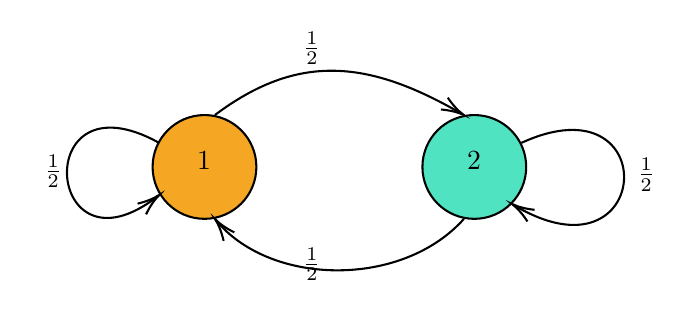
\begin{tikzpicture}[x=0.75pt,y=0.75pt,yscale=-1,xscale=1]
	%uncomment if require: \path (0,300); %set diagram left start at 0, and has height of 300
	
	%Shape: Circle [id:dp10052394937221254] 
	\draw  [fill={rgb, 255:red, 245; green, 166; blue, 35 }  ,fill opacity=1 ] (110,105) .. controls (110,91.19) and (121.19,80) .. (135,80) .. controls (148.81,80) and (160,91.19) .. (160,105) .. controls (160,118.81) and (148.81,130) .. (135,130) .. controls (121.19,130) and (110,118.81) .. (110,105) -- cycle ;
	%Shape: Circle [id:dp9437193586251307] 
	\draw  [fill={rgb, 255:red, 80; green, 227; blue, 194 }  ,fill opacity=1 ] (240,105) .. controls (240,91.19) and (251.19,80) .. (265,80) .. controls (278.81,80) and (290,91.19) .. (290,105) .. controls (290,118.81) and (278.81,130) .. (265,130) .. controls (251.19,130) and (240,118.81) .. (240,105) -- cycle ;
	%Curve Lines [id:da17352138739767575] 
	\draw    (140,80) .. controls (179.6,50.3) and (213.32,53.02) .. (258.62,79.2) ;
	\draw [shift={(260,80)}, rotate = 210.34] [color={rgb, 255:red, 0; green, 0; blue, 0 }  ][line width=0.75]    (10.93,-3.29) .. controls (6.95,-1.4) and (3.31,-0.3) .. (0,0) .. controls (3.31,0.3) and (6.95,1.4) .. (10.93,3.29)   ;
	%Curve Lines [id:da2659131152083798] 
	\draw    (141.59,131.91) .. controls (168.23,162.45) and (230.6,163.07) .. (260,130) ;
	\draw [shift={(140,130)}, rotate = 51.62] [color={rgb, 255:red, 0; green, 0; blue, 0 }  ][line width=0.75]    (10.93,-3.29) .. controls (6.95,-1.4) and (3.31,-0.3) .. (0,0) .. controls (3.31,0.3) and (6.95,1.4) .. (10.93,3.29)   ;
	%Curve Lines [id:da5459168562000609] 
	\draw    (113,93.33) .. controls (50.31,58.59) and (57.92,161.7) .. (112.51,119.07) ;
	\draw [shift={(113.33,118.41)}, rotate = 141.3] [color={rgb, 255:red, 0; green, 0; blue, 0 }  ][line width=0.75]    (10.93,-3.29) .. controls (6.95,-1.4) and (3.31,-0.3) .. (0,0) .. controls (3.31,0.3) and (6.95,1.4) .. (10.93,3.29)   ;
	%Curve Lines [id:da26931738393220694] 
	\draw    (287.67,93.41) .. controls (356.99,61.57) and (351.39,163.71) .. (284.02,123.36) ;
	\draw [shift={(283,122.74)}, rotate = 31.58] [color={rgb, 255:red, 0; green, 0; blue, 0 }  ][line width=0.75]    (10.93,-3.29) .. controls (6.95,-1.4) and (3.31,-0.3) .. (0,0) .. controls (3.31,0.3) and (6.95,1.4) .. (10.93,3.29)   ;
	
	% Text Node
	\draw (130,96) node [anchor=north west][inner sep=0.75pt]   [align=left] {1};
	% Text Node
	\draw (260,96) node [anchor=north west][inner sep=0.75pt]   [align=left] {2};
	% Text Node
	\draw (56.33,97.73) node [anchor=north west][inner sep=0.75pt]   {$\frac{1}{2}$};
	% Text Node
	\draw (342,99.4) node [anchor=north west][inner sep=0.75pt]  {$\frac{1}{2}$};
	% Text Node
	\draw (181,38.4) node [anchor=north west][inner sep=0.75pt]  {$\frac{1}{2}$};
	% Text Node
	\draw (181,142.4) node [anchor=north west][inner sep=0.75pt]   {$\frac{1}{2}$};
	
	
\end{tikzpicture}
\end{figure}